\documentclass[letter,11pt]{article}

\usepackage[spanish,es-nodecimaldot]{babel}
\usepackage[utf8]{inputenc}

\usepackage{lmodern}
\usepackage[T1]{fontenc}
\usepackage{textcomp}

\usepackage[svgnames]{xcolor}
\colorlet{shadecolor}{Gainsboro!50}

\usepackage[labelfont=bf]{caption}
\usepackage{graphicx}
\usepackage{pstricks}

\usepackage{anysize}
\marginsize{3cm}{2cm}{2cm}{3cm}

\usepackage{url}
\usepackage{siunitx}
\usepackage{amsmath}
\usepackage{array}

\usepackage{caption}
\newcommand{\source}[1]{\vspace{-11pt} \caption*{\small{\textbf{Nota:} {#1}}}}

\usepackage{fancyhdr}
\usepackage{lastpage}
\pagestyle{fancy}
\fancyhf{}
\fancyhead[LE,RO]{Laboratorio de Física Básica II}
\fancyfoot[CO,CE]{\thepage\ de \pageref{LastPage}}

\special{papersize=215.9mm,279.4mm}

\usepackage[
    pdfauthor={Carlos Eduardo Caballero Burgoa},%
    pdftitle={Laboratorio de Física Básica II},%
    pdfsubject={Constante elástica del resorte},%
    colorlinks,%
    citecolor=black,%
    filecolor=black,%
    linkcolor=black,%
    urlcolor=black,
    breaklinks]{hyperref}
\usepackage{breakurl}

\newcommand{\blankpage}{
\newpage
\thispagestyle{empty}
\mbox{}
\newpage
}

\renewcommand{\arraystretch}{1.2}

\title{Informe 2: Constante elástica del resorte}
\author{Carlos Eduardo Caballero Burgoa \\
    \small{\href{mailto:200201226@est.umss.edu}{200201226@est.umss.edu}}
}
\date{\today}

\begin{document}

\maketitle
\begin{center}
    \textbf{Grupo}: J2\\
    \textbf{Docente}: Ing. Milka Mónica Torrico Troche\\
    \textbf{Carrera}: Ing. Electromecánica
\end{center}

\begin{abstract}
Este documento detalla el experimento realizado en simulador para hallar la
constante de proporcionalidad de dos resortes a partir de la ley de
\emph{Hooke}, para esto se realizó la medición de la elongación de un resorte a
diferentes cantidades de masas disponibles; y posteriormente se calculó la 
relación funcional con el método de mínimos cuadrados, finalmente se determinó
el valor de la constante, resultando ser: $(4.00 \pm 0.02)[N/m]; 0.55\%$ para el
primer resorte y $(10.9 \pm 0.1)[N/m]; 1.18\%$ para el segundo.
\end{abstract}

\section{Introducción}

\begin{figure}
\centering
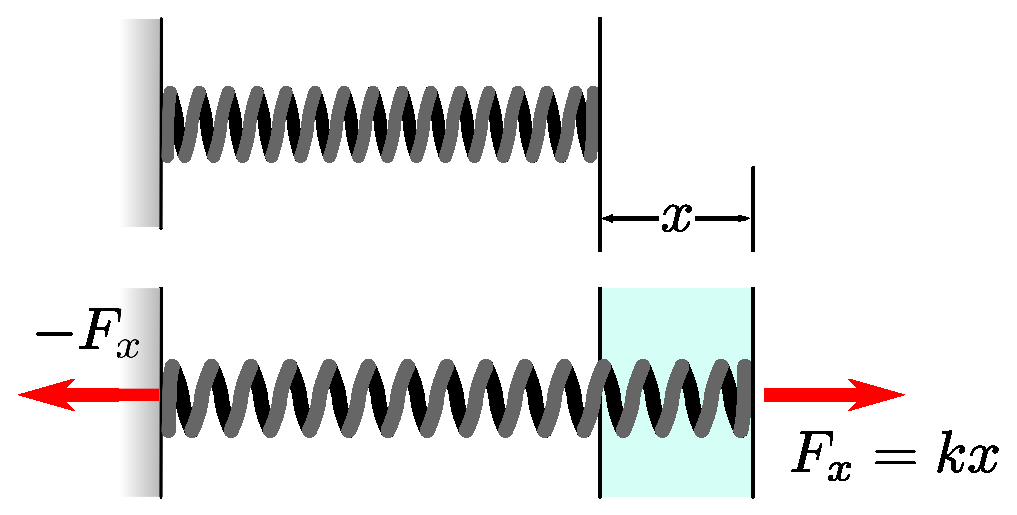
\includegraphics[width=0.38\textwidth]{resources/f1.eps}
\caption{Fuerza necesaria para estirar un resorte.}
\label{figura1}
\source{Física Universitaria Volumen I (p. 188), \\
Young, Hugh D. y Freedman, Roger A., 2013, Pearson.}
\end{figure}

Para mantener un resorte estirado una distancia $x$ más allá de su longitud sin
estirar, se debe aplicar una fuerza de igual magnitud en cada extremo como en la
\textbf{Figura \ref{figura1}}. Si el alargamiento $x$ no es excesivo, la fuerza
aplicada al extremo derecho tiene una componente $x$ directamente proporcional
a $x$, esto se conoce como la ley de \emph{Hooke}:

\begin{equation}
    \vec{F}_x = - k \vec{x}
\label{hooke}
\end{equation}
\vspace{0.10cm}

Donde $k$ es una constante llamada \textbf{constante de fuerza} (o constante de
resorte). Las unidades de $k$ son de fuerza dividida entre distancia: $[N/m]$ en
el sistema internacional \cite{Young&Freedman}.

Para el experimento se verificará la \textbf{Ecuación \ref{hooke}}.
A partir de la toma de datos de elongación y fuerza, se graficaron los datos, y
finalmente se determinarán las constantes de los resortes usados.

\section{Método experimental}

\begin{figure}
\centering
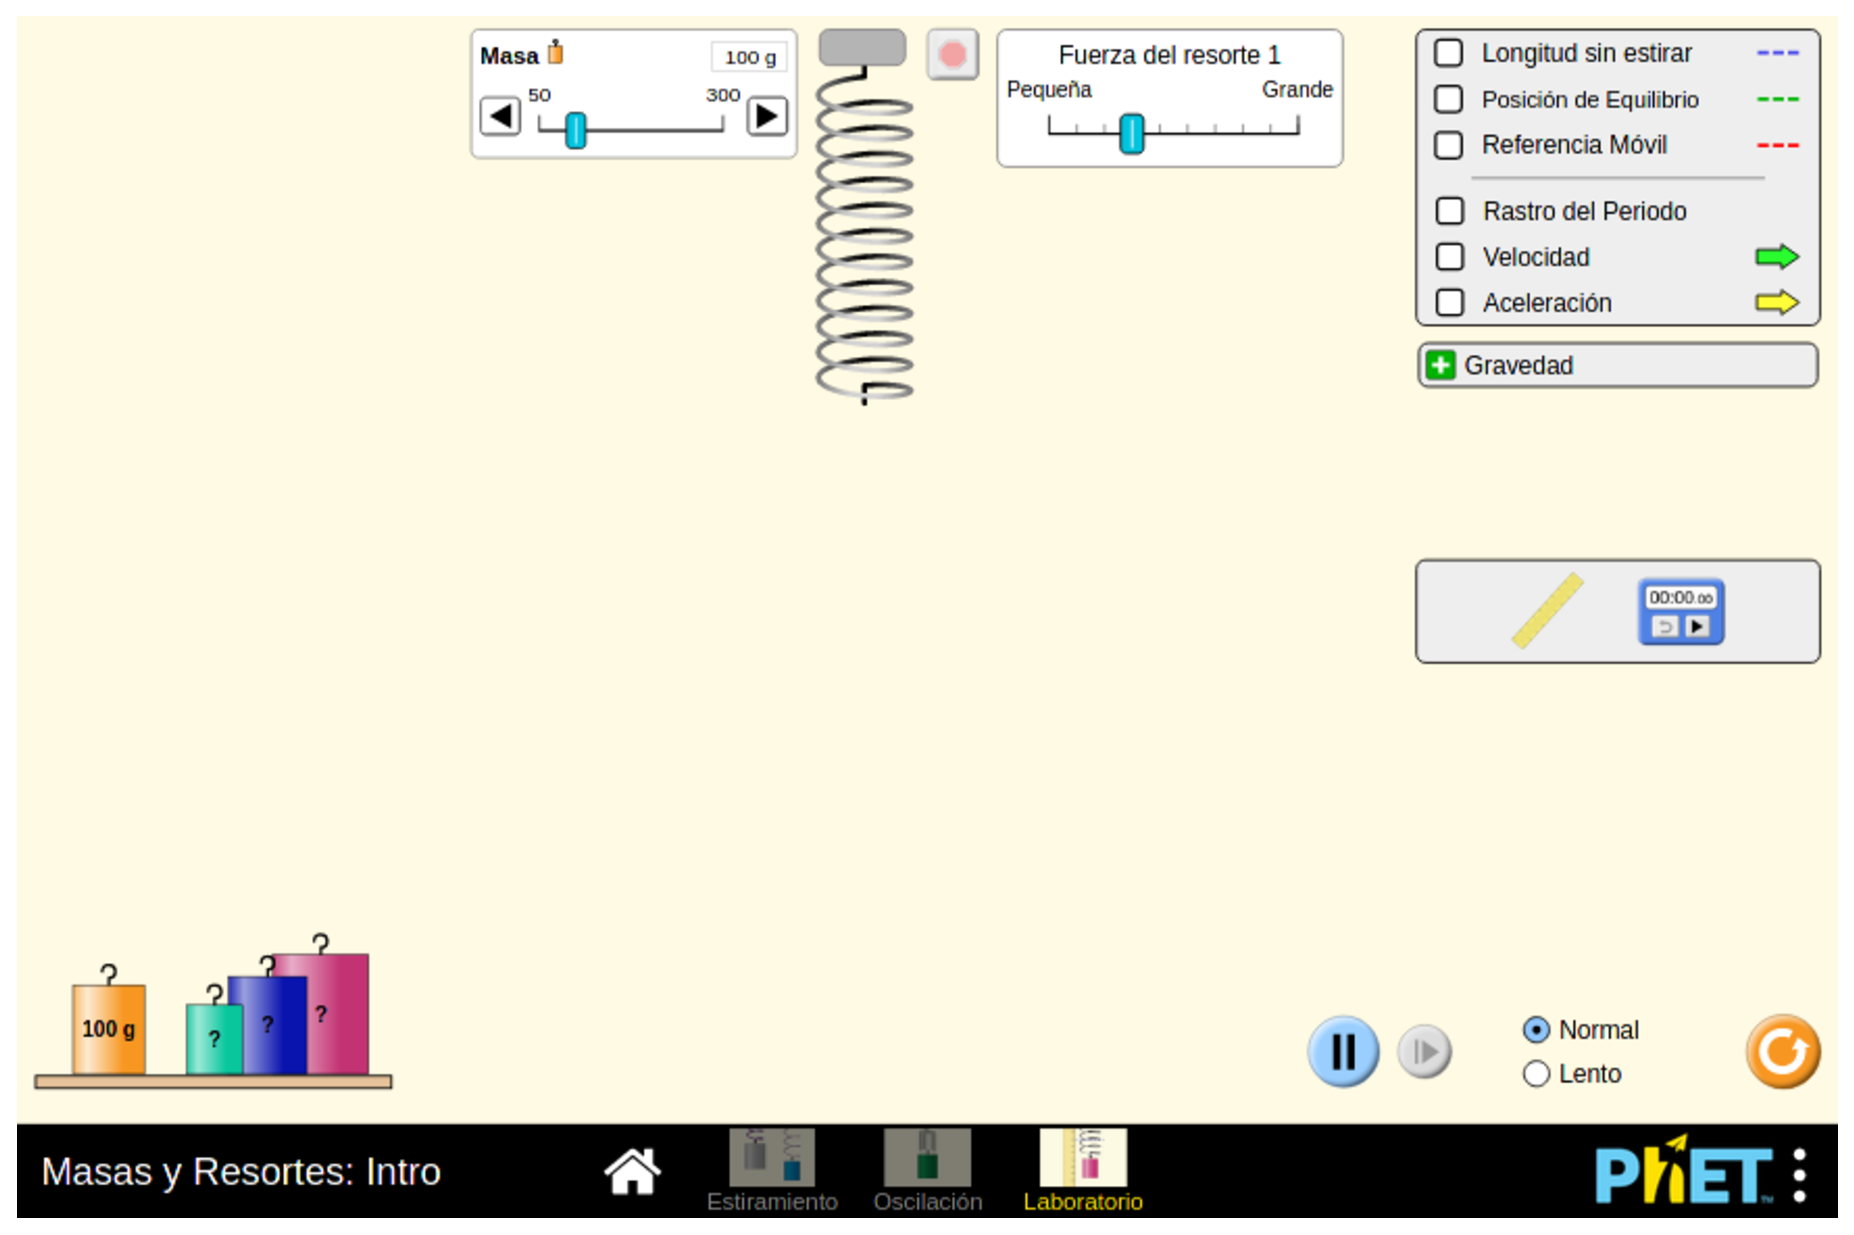
\includegraphics[width=0.90\textwidth]{resources/f2.eps}
\caption{Simulador de resortes.}
\label{figura2}
\source{Fotografía propia.}
\end{figure}

Para la realización del experimento, se emplea el simulador de resortes de
\emph{PHET}, ubicado en la dirección web: \url{
https://phet.colorado.edu/sims/html/masses-and-springs-basics/latest/masses-and-springs-basics_es.html
}, tal como se presenta en la \textbf{Figura \ref{figura2}}.

Para el simulador se escoge una fuerza del resorte, que se mantendrá constante
durante la medición, y se registrarán diferentes valores de masa ($m$) para
medir su variación de longitud ($x$).

Una vez medidos los datos para dos resortes con diferente fuerza del resorte,
se procederá a graficar la relación fuerza vs. longitud del resorte, y con la
ayuda del método de los mínimos cuadrados, se halla la relación funcional entre
las variables.

\subsection{Resorte pequeño}

En el \textbf{Cuadro \ref{cuadro1}}, se pueden ver los valores tomados del 
experimento, tanto la masa como la longitud de la deformación resultante, para
una fuerza del resorte pequeño.

\begin{table}[!h]
\begin{center}
\begin{tabular}{|c||>{\centering}m{2.0cm}<{\centering}
                  |>{\centering}m{2.0cm}<{\centering}|
                |c||>{\centering}m{2.0cm}<{\centering}
                  |>{\centering}m{2.0cm}<{\centering}|}
\hline
$i$ & $m_i [g]$ & $x_i [cm]$ & $i$ & $m_i [g]$ & $x_i [cm]$
    \tabularnewline \hline \hline
 1 &   0 & 47 & 10 & 130 & 79 \tabularnewline \hline
 2 &  50 & 60 & 11 & 140 & 82 \tabularnewline \hline
 3 &  60 & 62 & 12 & 150 & 84 \tabularnewline \hline
 4 &  70 & 65 & 13 & 160 & 86 \tabularnewline \hline
 5 &  80 & 67 & 14 & 170 & 89 \tabularnewline \hline
 6 &  90 & 69 & 15 & 180 & 91 \tabularnewline \hline
 7 & 100 & 72 & 16 & 190 & 94 \tabularnewline \hline
 8 & 110 & 74 & 17 & 200 & 96 \tabularnewline \hline
 9 & 120 & 77 & 18 & 210 & 99 \tabularnewline \hline
\end{tabular}
\caption{Mediciones de longitud en función de \\
la masa provista (Resorte pequeño).}
\label{cuadro1}
\source{Elaboración propia.}
\end{center}
\end{table}

\subsection{Resorte grande}

En el \textbf{Cuadro \ref{cuadro2}}, pueden ver los valores tomados del 
experimento, tanto la masa como la longitud de la deformación resultante, para
una fuerza del resorte grande.

\begin{table}[!h]
\begin{center}
\begin{tabular}{|c||>{\centering}m{2.0cm}<{\centering}
                  |>{\centering}m{2.0cm}<{\centering}|
                |c||>{\centering}m{2.0cm}<{\centering}
                  |>{\centering}m{2.0cm}<{\centering}|}
\hline
$i$ & $m_i [g]$ & $x_i [cm]$ & $i$ & $m_i [g]$ & $x_i [cm]$
    \tabularnewline \hline \hline
 1 &   0 & 47 & 10 & 220 & 67 \tabularnewline \hline
 2 & 140 & 60 & 11 & 230 & 68 \tabularnewline \hline
 3 & 150 & 61 & 12 & 240 & 69 \tabularnewline \hline
 4 & 160 & 61 & 13 & 250 & 70 \tabularnewline \hline
 5 & 170 & 62 & 14 & 260 & 70 \tabularnewline \hline
 6 & 180 & 63 & 15 & 270 & 71 \tabularnewline \hline
 7 & 190 & 64 & 16 & 280 & 72 \tabularnewline \hline
 8 & 200 & 65 & 17 & 290 & 73 \tabularnewline \hline
 9 & 210 & 66 & 18 & 300 & 74 \tabularnewline \hline
\end{tabular}
\caption{Mediciones de longitud en función de \\
la masa provista (Resorte grande).}
\label{cuadro2}
\source{Elaboración propia.}
\end{center}
\end{table}

\section{Resultados}

\subsection{Resorte pequeño}

\begin{figure}
\centering
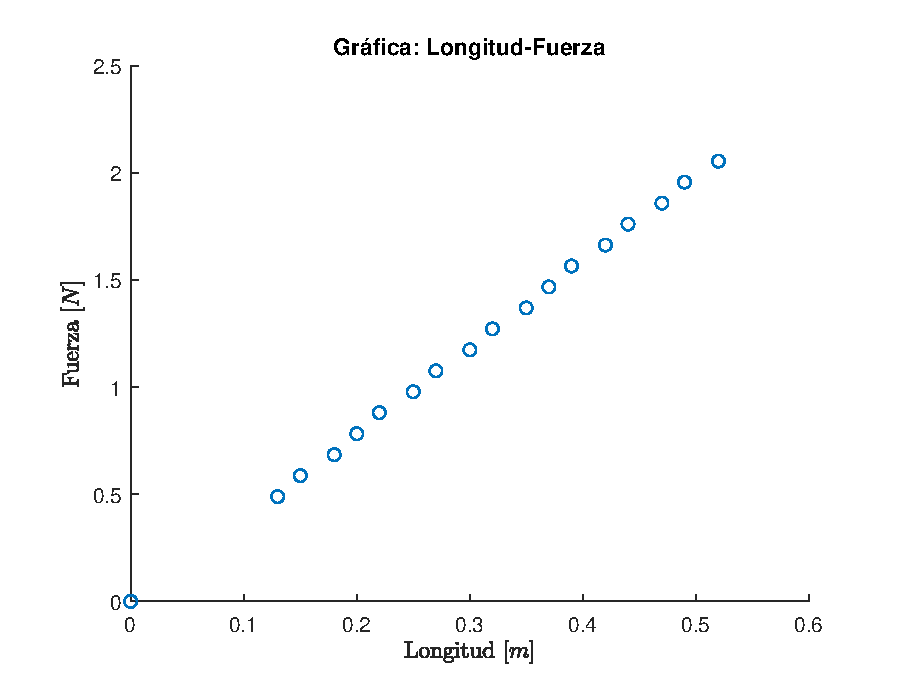
\includegraphics[width=0.80\textwidth]{resources/m1.eps}
\caption{Gráfica de longitud vs fuerza (Resorte pequeño).}
\label{figura3}
\source{Elaboración propia.}
\end{figure}

A partir de los datos obtenidos se genera la gráfica de la
\textbf{Figura \ref{figura3}}.

Posteriormente se calculo la recta de mejor ajuste por el método de los mínimos
cuadrados, resultando los siguientes valores:

\begin{equation*}
    A = (-0.016 \pm 0.007) [N]; 46.89\%
\end{equation*}
\begin{equation*}
    B = (4.00 \pm 0.02) [N/m]; 0.55\%
\end{equation*}
\vspace{0.10cm}

Siendo su coeficiente de correlación ($r$):

\begin{equation*}
    r = 0.9998
\end{equation*}
\vspace{0.10cm}

Considerando que el modelo de ajuste es:

\begin{equation*}
    F = A + B x
\end{equation*}
\vspace{0.10cm}

Por tanto la relación funcional entre $F$ y $x$, es:

\begin{equation*}
    F \propto x
\end{equation*}
\vspace{0.10cm}

Verificándose el comportamiento establecido por la
\textbf{Ecuación \ref{hooke}}.

La constante elástica para el resorte pequeño del experimento es:

\begin{equation*}
    k = (4.00 \pm 0.02) [N/m]; 0.55\%
\end{equation*}
\vspace{0.10cm}

\subsection{Resorte grande}

\begin{figure}
\centering
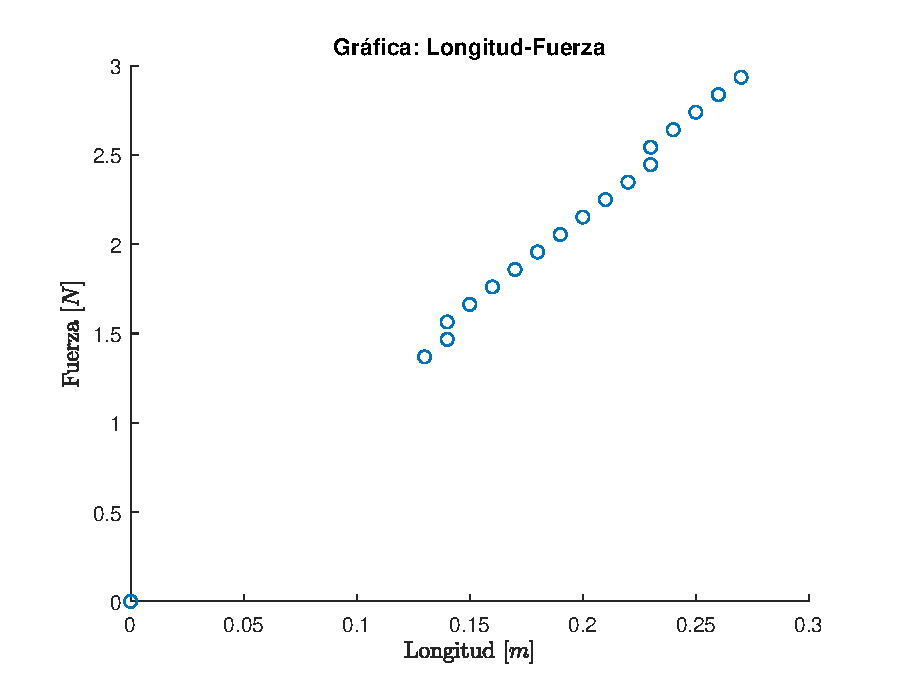
\includegraphics[width=0.80\textwidth]{resources/m2.eps}
\caption{Gráfica de longitud vs fuerza (Resorte grande).}
\label{figura4}
\source{Elaboración propia.}
\end{figure}

A partir de los datos obtenidos se genera la gráfica de la
\textbf{Figura \ref{figura4}}.

Posteriormente se calculo la recta de mejor ajuste por el método de los mínimos
cuadrados, resultando los siguientes valores:

\begin{equation*}
    A = (-0.01 \pm 0.02) [N]; 330.46\%
\end{equation*}
\begin{equation*}
    B = (10.9 \pm 0.1) [N/m]; 1.18\%
\end{equation*}
\vspace{0.10cm}

Siendo su coeficiente de correlación ($r$):

\begin{equation*}
    r = 0.9989
\end{equation*}
\vspace{0.10cm}

Considerando que el modelo de ajuste es:

\begin{equation*}
    F = A + B x
\end{equation*}
\vspace{0.10cm}

Por tanto la relación funcional entre $F$ y $x$, es:

\begin{equation*}
    F \propto x
\end{equation*}
\vspace{0.10cm}

La constante elástica para el resorte grande del experimento es:

\begin{equation*}
    k = (10.9 \pm 0.1) [N/m]; 1.18\%
\end{equation*}
\vspace{0.10cm}

\section{Discusión}

Puede notarse que en ambos resortes la variable $a$ es negativa, además que
el error de $b$ es pequeño, ambas son reflejo del uso de un simulador, ya que se
están tratando con resortes ideales.

\section{Conclusiones}

Se halló la relación funcional entre el incremento de la longitud del resorte y
la fuerza aplicada, verificándose así la ley de \emph{Hooke}.

También se calculó el valor de la constante elástica del resorte.

\begin{thebibliography}{99}

\bibitem{Young&Freedman} Young, Hugh D. y Freedman, Roger A. (2013).\\
Física Universitaria. Volumen 1.\\
13va Edición.\\
Capitulo 11.

\end{thebibliography}

\newpage
\section*{Apéndice: Cálculos adicionales}

\subsection{Resorte pequeño}

Conociendo $m_i$, $x_i$, y $g$, se detallan los valores de la fuerza calculada
($F$) y la longitud del estiramiento del resorte pequeño ($\Delta x$) en el
\textbf{Cuadro \ref{cuadro3}}.

\begin{table}[!h]
\begin{center}
\begin{tabular}{|c||>{\centering}m{2.0cm}<{\centering}
                  |>{\centering}m{2.0cm}<{\centering}|
                |c||>{\centering}m{2.0cm}<{\centering}
                  |>{\centering}m{2.0cm}<{\centering}|}
\hline
$i$ & $F_i [N]$ & $\Delta x_i [m]$ & $i$ & $F_i [N]$ & $\Delta x_i [m]$
    \tabularnewline \hline \hline
 1 & $     0$ & $     0$ & 10 & $1.2714$ & $0.3200$\tabularnewline \hline
 2 & $0.4890$ & $0.1300$ & 11 & $1.3692$ & $0.3500$\tabularnewline \hline
 3 & $0.5868$ & $0.1500$ & 12 & $1.4670$ & $0.3700$\tabularnewline \hline
 4 & $0.6846$ & $0.1800$ & 13 & $1.5648$ & $0.3900$\tabularnewline \hline
 5 & $0.7824$ & $0.2000$ & 14 & $1.6626$ & $0.4200$\tabularnewline \hline
 6 & $0.8802$ & $0.2200$ & 15 & $1.7604$ & $0.4400$\tabularnewline \hline
 7 & $0.9780$ & $0.2500$ & 16 & $1.8582$ & $0.4700$\tabularnewline \hline
 8 & $1.0758$ & $0.2700$ & 17 & $1.9560$ & $0.4900$\tabularnewline \hline
 9 & $1.1736$ & $0.3000$ & 18 & $2.0538$ & $0.5200$\tabularnewline \hline
\end{tabular}
\caption{Calculo de la fuerza y la longitud (Resorte pequeño).}
\label{cuadro3}
\source{Elaboración propia.}
\end{center}
\end{table}

Se calculan los parámetros de la recta por el método de los mínimos cuadrados,
con la ayuda de los datos presentados en el \textbf{Cuadro \ref{cuadro4}}.

\begin{table}[!h]
\begin{center}
\begin{tabular}{|c||>{\centering}m{1.8cm}<{\centering}
                  |>{\centering}m{1.8cm}<{\centering}
                  |>{\centering}m{1.8cm}<{\centering}|
                  |>{\centering}m{1.8cm}<{\centering}
                  |>{\centering}m{1.8cm}<{\centering}
                  |>{\centering}m{2.1cm}<{\centering}|}
\hline
$i$ & $x_i y_i$ & $x^2_i$ & $y^2_i$ & $Y_i$ & $d_i$ & $d^2_i\,(\num{e-3})$
    \tabularnewline \hline \hline
 1 &      0 &      0 &      0 & -0.0157 &  0.0157 & 0.2475
    \tabularnewline \hline
 2 & 0.0636 & 0.0169 & 0.2391 &  0.5047 & -0.0157 & 0.245
    \tabularnewline \hline
 3 & 0.0880 & 0.0225 & 0.3443 &  0.5847 &  0.0021 & 0.004
    \tabularnewline \hline
 4 & 0.1232 & 0.0324 & 0.4687 &  0.7048 & -0.0202 & 0.4091
    \tabularnewline \hline
 5 & 0.1565 & 0.0400 & 0.6121 &  0.7849 & -0.0025 & 0.0062
    \tabularnewline \hline
 6 & 0.1936 & 0.0484 & 0.7748 &  0.8650 &  0.0152 & 0.2325
    \tabularnewline \hline
 7 & 0.2445 & 0.0625 & 0.9565 &  0.9850 & -0.0070 & 0.0496
    \tabularnewline \hline
 8 & 0.2905 & 0.0729 & 1.1573 &  1.0651 &  0.0107 & 0.1144
    \tabularnewline \hline
 9 & 0.3521 & 0.0900 & 1.3773 &  1.1852 & -0.0116 & 0.1345
    \tabularnewline \hline
10 & 0.4068 & 0.1024 & 1.6165 &  1.2653 &  0.0061 & 0.0377
    \tabularnewline \hline
11 & 0.4792 & 0.1225 & 1.8747 &  1.3854 & -0.0162 & 0.2610
    \tabularnewline \hline
12 & 0.5428 & 0.1369 & 2.1521 &  1.4654 &  0.0016 & 0.0025
    \tabularnewline \hline
13 & 0.6103 & 0.1521 & 2.4486 &  1.5455 &  0.0193 & 0.3733
    \tabularnewline \hline
14 & 0.6983 & 0.1764 & 2.7642 &  1.6656 & -0.0030 & 0.0088
    \tabularnewline \hline
15 & 0.7746 & 0.1936 & 3.0990 &  1.7456 &  0.0148 & 0.2180
    \tabularnewline \hline
16 & 0.8734 & 0.2209 & 3.4529 &  1.8657 & -0.0075 & 0.0567
    \tabularnewline \hline
17 & 0.9584 & 0.2401 & 3.8259 &  1.9458 &  0.0102 & 0.104
    \tabularnewline \hline
18 & 1.0680 & 0.2704 & 4.2181 &  2.0659 & -0.0121 & 0.146
    \tabularnewline \hline
\end{tabular}
\caption{Valores para el método de mínimos cuadrados (Resorte pequeño).}
\label{cuadro4}
\source{Elaboración propia.}
\end{center}
\end{table}

\begin{equation*}
    n = 18
\end{equation*}
\begin{equation*}
    \sum x_i = 5.4700
\end{equation*}
\begin{equation*}
    \sum y_i = 21.6138
\end{equation*}
\begin{equation*}
    \sum x^2_i = 2.0009
\end{equation*}
\begin{equation*}
    \sum y^2_i = 31.3822
\end{equation*}
\begin{equation*}
    \sum x_i y_i = 7.9238
\end{equation*}
\begin{equation*}
    \Delta_1 = n \sum x^2_i - \left( \sum x_i \right)^2 = 6.0953
\end{equation*}
\begin{equation*}
    \Delta_2 = n \sum y^2_i - \left( \sum y_i \right)^2 = 97.7240
\end{equation*}
\begin{equation*}
    A = \frac{\sum y_i \sum x^2_i - \sum x_i y_i \sum x_i}{\Delta_1} = -0.0157
\end{equation*}
\begin{equation*}
    B = \frac{n \sum x_i y_i - \sum x_i \sum y_i}{\Delta_1} = 4.0031
\end{equation*}
\begin{equation*}
    \sum d^2 = 0.0027
\end{equation*}
\begin{equation*}
    \sigma^2 = \frac{\sum d^2_i}{n-2} = \num{1.6575e-4}
\end{equation*}
\begin{equation*}
    \sigma_A = \sqrt{\frac{\sigma^2 \sum x^2_i}{\Delta_1}} = 0.0074
\end{equation*}
\begin{equation*}
    \sigma_B = \sqrt{\frac{\sigma^2 n}{\Delta_1}} = 0.0221
\end{equation*}
\vspace{0.10cm}

Parámetros de la recta obtenida:

\begin{equation*}
    A = (-0.0157 \pm 0.0074) [N]; 46.8866\%
\end{equation*}
\begin{equation*}
    B = (4.0031 \pm 0.0221) [N/m]; 0.5527\%
\end{equation*}
\vspace{0.10cm}

Siendo el coeficiente de correlación:

\begin{equation*}
    R = \frac{n \sum x_i y_i - (\sum x_i)(\sum y_i)}{\sqrt{\Delta_1 \Delta_2}}
      = 0.9998
\end{equation*}
\vspace{0.10cm}

La ecuación de la recta resultante es:

\begin{equation*}
    y = -0.0157 + 4.0031\,x
\end{equation*}
\vspace{0.10cm}

\subsection{Resorte grande}

Conociendo $m_i$, $x_i$, y $g$, se detallan los valores de la fuerza calculada
($F$) y la longitud del estiramiento del resorte grande ($\Delta x$) en el
\textbf{Cuadro \ref{cuadro5}}.

\begin{table}[!h]
\begin{center}
\begin{tabular}{|c||>{\centering}m{2.0cm}<{\centering}
                  |>{\centering}m{2.0cm}<{\centering}|
                |c||>{\centering}m{2.0cm}<{\centering}
                  |>{\centering}m{2.0cm}<{\centering}|}
\hline
$i$ & $F_i [N]$ & $\Delta x_i [m]$ & $i$ & $F_i [N]$ & $\Delta x_i [m]$
    \tabularnewline \hline \hline
 1 & $     0$ & $     0$ & 10 & $2.1516$ & $0.2000$\tabularnewline \hline
 2 & $1.3692$ & $0.1300$ & 11 & $2.2494$ & $0.2100$\tabularnewline \hline
 3 & $1.4670$ & $0.1400$ & 12 & $2.3472$ & $0.2200$\tabularnewline \hline
 4 & $1.5648$ & $0.1400$ & 13 & $2.4450$ & $0.2300$\tabularnewline \hline
 5 & $1.6626$ & $0.1500$ & 14 & $2.5428$ & $0.2300$\tabularnewline \hline
 6 & $1.7604$ & $0.1600$ & 15 & $2.6406$ & $0.2400$\tabularnewline \hline
 7 & $1.8582$ & $0.1700$ & 16 & $2.7384$ & $0.2500$\tabularnewline \hline
 8 & $1.9560$ & $0.1800$ & 17 & $2.8362$ & $0.2600$\tabularnewline \hline
 9 & $2.0538$ & $0.1900$ & 18 & $2.9340$ & $0.2700$\tabularnewline \hline
\end{tabular}
\caption{Calculo de la fuerza y la longitud (Resorte grande).}
\label{cuadro5}
\source{Elaboración propia.}
\end{center}
\end{table}

Se calculan los parámetros de la recta por el método de los mínimos cuadrados,
con la ayuda de los datos presentados en el \textbf{Cuadro \ref{cuadro6}}.

\begin{table}[!h]
\begin{center}
\begin{tabular}{|c||>{\centering}m{1.8cm}<{\centering}
                  |>{\centering}m{1.8cm}<{\centering}
                  |>{\centering}m{1.8cm}<{\centering}|
                  |>{\centering}m{1.8cm}<{\centering}
                  |>{\centering}m{1.8cm}<{\centering}
                  |>{\centering}m{2.1cm}<{\centering}|}
\hline
$i$ & $x_i y_i$ & $x^2_i$ & $y^2_i$ & $Y_i$ & $d_i$ & $d^2_i$
    \tabularnewline \hline \hline
 1 &      0 &      0 &      0 & -0.0076 &  0.0076 & 0.0001
    \tabularnewline \hline
 2 & 0.1780 & 0.0169 & 1.8747 &  1.4087 & -0.0395 & 0.0016
    \tabularnewline \hline
 3 & 0.2054 & 0.0196 & 2.1521 &  1.5176 & -0.0506 & 0.0026
    \tabularnewline \hline
 4 & 0.2191 & 0.0196 & 2.4486 &  1.5176 &  0.0472 & 0.0022
    \tabularnewline \hline
 5 & 0.2494 & 0.0225 & 2.7642 &  1.6265 &  0.0361 & 0.0013
    \tabularnewline \hline
 6 & 0.2817 & 0.0256 & 3.0990 &  1.7355 &  0.0249 & 0.0006
    \tabularnewline \hline
 7 & 0.3159 & 0.0289 & 3.4529 &  1.8444 &  0.0138 & 0.0002
    \tabularnewline \hline
 8 & 0.3521 & 0.0324 & 3.8259 &  1.9534 &  0.0026 & 0.0000
    \tabularnewline \hline
 9 & 0.3902 & 0.0361 & 4.2181 &  2.0623 & -0.0085 & 0.0001
    \tabularnewline \hline
10 & 0.4303 & 0.0400 & 4.6294 &  2.1713 & -0.0197 & 0.0004
    \tabularnewline \hline
11 & 0.4724 & 0.0441 & 5.0598 &  2.2802 & -0.0308 & 0.0009
    \tabularnewline \hline
12 & 0.5164 & 0.0484 & 5.5093 &  2.3892 & -0.0420 & 0.0018
    \tabularnewline \hline
13 & 0.5624 & 0.0529 & 5.9780 &  2.4981 & -0.0531 & 0.0028
    \tabularnewline \hline
14 & 0.5848 & 0.0529 & 6.4658 &  2.4981 &  0.0447 & 0.0020
    \tabularnewline \hline
15 & 0.6337 & 0.0576 & 6.9728 &  2.6071 &  0.0335 & 0.0011
    \tabularnewline \hline
16 & 0.6846 & 0.0625 & 7.4988 &  2.7160 &  0.0224 & 0.0005
    \tabularnewline \hline
17 & 0.7374 & 0.0676 & 8.0440 &  2.8250 &  0.0112 & 0.0001
    \tabularnewline \hline
18 & 0.7922 & 0.0729 & 8.6084 &  2.9339 &  0.0001 & 0.0000
    \tabularnewline \hline
\end{tabular}
\caption{Valores para el método de mínimos cuadrados (Resorte grande).}
\label{cuadro6}
\source{Elaboración propia.}
\end{center}
\end{table}

\begin{equation*}
    n = 18
\end{equation*}
\begin{equation*}
    \sum x_i = 3.3700
\end{equation*}
\begin{equation*}
    \sum y_i = 36.5772
\end{equation*}
\begin{equation*}
    \sum x^2_i = 0.7005
\end{equation*}
\begin{equation*}
    \sum y^2_i = 82.6020
\end{equation*}
\begin{equation*}
    \sum x_i y_i = 7.6059
\end{equation*}
\begin{equation*}
    \Delta_1 = n \sum x^2_i - \left( \sum x_i \right)^2 = 1.2521
\end{equation*}
\begin{equation*}
    \Delta_2 = n \sum y^2_i - \left( \sum y_i \right)^2 = 148.9437
\end{equation*}
\begin{equation*}
    A = \frac{\sum y_i \sum x^2_i - \sum x_i y_i \sum x_i}{\Delta_1} = -0.0076
\end{equation*}
\begin{equation*}
    B = \frac{n \sum x_i y_i - \sum x_i \sum y_i}{\Delta_1} = 10.8946
\end{equation*}
\begin{equation*}
    \sum d^2 = 0.0183
\end{equation*}
\begin{equation*}
    \sigma^2 = \frac{\sum d^2_i}{n-2} = 0.0011
\end{equation*}
\begin{equation*}
    \sigma_A = \sqrt{\frac{\sigma^2 \sum x^2_i}{\Delta_1}} = 0.0253
\end{equation*}
\begin{equation*}
    \sigma_B = \sqrt{\frac{\sigma^2 n}{\Delta_1}} = 0.1281
\end{equation*}
\vspace{0.10cm}

Parámetros de la recta obtenida:

\begin{equation*}
    A = (-0.0076 \pm 0.0253) [N]; 330.4569\%
\end{equation*}
\begin{equation*}
    B = (10.8946 \pm 0.1281) [N/m]; 1.1758\%
\end{equation*}
\vspace{0.10cm}

Siendo el coeficiente de correlación:

\begin{equation*}
    R = \frac{n \sum x_i y_i - (\sum x_i)(\sum y_i)}{\sqrt{\Delta_1 \Delta_2}}
      = 0.9989
\end{equation*}
\vspace{0.10cm}

La ecuación de la recta resultante es:

\begin{equation*}
    y = -0.0076 + 10.8946\,x
\end{equation*}
\vspace{0.10cm}

\end{document}

